%Problem mit der �berschrift: Binomische Formeln
\chapter*{Funktionen}
%Autor: Katja Matthes
\section*{Lineare Funktionen $y = f(x) = mx+n$}
\begin{itemize}
	\item \textbf{Definitionsbereich}: $ D = \mathbb{R} $
	\item \textbf{Wertebereich}: $ W = \mathbb{R} $
	\item \textbf{Nullstelle}: $ x_0 = -\frac{n}{m} $
	\item \textbf{Anstieg}: $ m = tan \ \alpha = \frac{y_2 - y_1}{x_2 x_1}
$
	\item \textbf{Schnittpunkt mir der y-Achse}:\\ $ S_y = (0;n) $
	\item \textbf{Graph}: $f$: $m =1$, $n=0$; $g$: $m=1$, $n=2$; $h$: $m=
-2$, $n=2$ \\
\end{itemize}
		\includegraphics[width=.6\textwidth]{img/LinF.jpg}

\section*{Quadratische Funktionen}
\subsection*{Allgemeine Form: $y= ax^2 + bx + c$}
\begin{itemize}
	\item \textbf{Definitionsbereich}: $ D = \mathbb{R} $
	\item \textbf{Wertebereich für $a>0$}: $ W = [\frac{4ac-b^2}{4a}, +\infty) $
	\item \textbf{Wertebereich für $a<0$}: $ W = (-\infty, \frac{4ac-b^2}{4a}] $
	\item \textbf{Nullstelle}: $ x_{1,2} \ = \ \frac {-b \ \pm \ \sqrt{b^2 \ - \ 4ac}} {2a} $
	\item \textbf{Scheitelpunkt}: $ x_{1,2} \ = \ S(-\frac{b}{2a}, \frac{4ac-b^2}{4a} )$
\end{itemize}

\subsection*{Normalform $y = x^2 + px + q$}
\begin{itemize}
	\item \textbf{Definitionsbereich}: $ D = \mathbb{R} $
	\item \textbf{Wertebereich}: $ W = [q-\frac{p^2}{4}, +\infty) $
	\item \textbf{Nullstelle}: $ x_{1, 2}= - \frac{p}{2} \pm
\sqrt{\frac{p^2}{a}-q} $
	\item \textbf{Scheitelpunkt}: $ S(-\frac{p}{2}, -\frac{p^2}{4}+q )$
	\item \textbf{Spezialfall}: $y = (x+d)^2 +e $
	\item \textbf{Graph}: \\
		$f$: $a=\frac 1 2$, $b=-2$, $c=2$; \\
		$g$: $a=1$, $b=0$, $c=0$; \\
		$h$: $a=-4$, $b=0$, $c=-\frac 1 2$ \\
\end{itemize}
%\textbf{Graph}: \\
%		$f$: $a=\frac 1 2$, $b=-2$, $c=2$; \\
%		$g$: $a=1$, $b=0$, $c=0$; \\
%		$h$: $a=-4$, $b=0$, $c=-\frac 1 2$ \\
	\includegraphics[width=.6\textwidth]{img/QuadFkt.jpg}

\section*{Potenzfunktionen $ y = f(x) = x^n $}

\subsection*{Positiver gerader Exponent\\ $n = 2m$ mit $ m \in \mathbb{N}-\{0\}$}
\begin{itemize}
	\item \textbf{Definitionsbereich}: $ D = \mathbb{R} $
	\item \textbf{Wertebereich}: $ W = [0, + \infty) $
	\item \textbf{Nullstelle}: $ x_0 = 0 $
	\item \textbf{gemeinsame Punkte}: $(-1;1), (0;0), (1;1) $
	\item \textbf{Graph}: $f$: $n=2$; $g$: $n=4$; $h$: $n=8$ \\ 
\begin{center}
	\includegraphics[width=0.60\textwidth]{img/P1.jpg}
\end{center}
\end{itemize}

\subsection*{Positiver ungerader Exponent\\ $n = 2m+1$ mit $ m \in \mathbb{N}-\{0\}$}
\begin{minipage}{.5\textwidth}
\begin{itemize}
	\item \textbf{Definitionsbereich}: $ D = \mathbb{R} $
	\item \textbf{Wertebereich}: $ W = \mathbb{R} $
	\item \textbf{Nullstelle}: $ x_0 = 0 $
	\item \textbf{gemeinsame Punkte}:\\ $(-1;-1), (0;0), (1;1) $
	\item \textbf{Graph}: $f$: $n = 3$; $g$: $n=9$ \\
\end{itemize}
\end{minipage}
\begin{minipage}{.5\textwidth}
		\includegraphics[height=4cm]{img/P2.jpg}
\end{minipage}


\subsection*{Negativer gerader Exponent\\ $n = -2m$ mit $ m \in \mathbb{N}-\{0\}$}
\begin{itemize}
	\item \textbf{Definitionsbereich}: $ D = \mathbb{R}-\{0\} $
	\item \textbf{Wertebereich}: $ W = (0, + \infty) $
	\item \textbf{Nullstelle}: keine
	\item \textbf{gemeinsame Punkte}: $(-1;1), (1;1) $
	\item \textbf{Graph}:$f$: $n = -2$; $g$: $n=-8$ \\
\begin{center}
		\includegraphics[width=0.60\textwidth]{img/P3.jpg}
\end{center}
\end{itemize}

\subsection*{Negativer ungerader Exponent\\ $n = -(2m+1)$ mit $ m \in \mathbb{N}-\{0\}$}
\begin{itemize}
	\item \textbf{Definitionsbereich}: $ D = \mathbb{R}-\{0\} $
	\item \textbf{Wertebereich}: $ W = \mathbb{R}-\{0\} $
	\item \textbf{Nullstelle}: keine
	\item \textbf{gemeinsame Punkte}: $(-1;-1), (1;1) $
	\item \textbf{Graph}:$f$: $n = -3$; $g$: $n=-9$ \\
\begin{center}
		\includegraphics[width=0.60\textwidth]{img/P4.jpg}
\end{center}
\end{itemize}

\section*{Wurzelfunktionen $y = x^n $ mit $ n = \frac{p}{q}$ \\ ($p$, $q \in \mathbb{N}-\{0\}$, $ q $ teilt $ p $ nicht) }
\begin{itemize}
	\item \textbf{Definitionsbereich}: $ D = [0, +\infty) $
	\item \textbf{Wertebereich}: $ W = [0, +\infty) $
	\item \textbf{Nullstelle}: $x_0 = 0 $
	\item \textbf{gemeinsame Punkte}: $(0;0), (1;1) $
	\item \textbf{Graph}:$f$: $n = \frac{1}{2}$; $g$: $n=\frac{1}{4}$ \\
\begin{center}
		\includegraphics[width=0.60\textwidth]{img/WurzelF.jpg}
\end{center}
\end{itemize}

\section*{Winkelfunktionen}

\subsection*{Sinusfunktion $ y = \sin x $}
\begin{itemize}
	\item \textbf{Definitionsbereich}: $ D = \mathbb{R} $
	\item \textbf{Wertebereich}: $ W = [-1, +1] $
	\item \textbf{Nullstelle}: $x_k = k\pi $, $k \in \mathbb{Z}$
	\item \textbf{Periode}: $2\pi$
	\item \textbf{Graph}: \\
\begin{center}
		\includegraphics[width=0.60\textwidth]{img/SinF1.jpg}
\end{center}
\end{itemize}

\subsection*{Sinusfunktion $ y = a \sin (bx + c) $ \\ mit $ a $, $c \in \mathbb{R}$, $b \in \mathbb{R}-\{0\}$}
\begin{itemize}
	\item \textbf{Definitionsbereich}: $ D = \mathbb{R} $
	\item \textbf{Wertebereich}: $ W = [-a, +a] $
	\item \textbf{Nullstelle}: $x_k =  \frac{k\pi - c}{b} $, $k \in \mathbb{Z}$
	\item \textbf{Periode}: $\frac{2\pi}{b}$
	\item \textbf{Verschiebung in x-Richtung}: Verschiebung um $\frac{c}{b}$ ($> 0$) in negativer x-Richtung
	\item \textbf{Graph}:$f$: $a = 2$, $b=1$, $c=0$; $g$: $a=1$, $b=2$, $c=0$; $h$: $a=1$, $b=2$, $c=\pi$ \\
\begin{center}
		\includegraphics[width=0.60\textwidth]{img/SinF2.jpg}
\end{center}
\end{itemize}

\subsection*{Kosinusfunktion $y = \cos x$}
\begin{itemize}
	\item \textbf{Definitionsbereich}: $ D = \mathbb{R} $
	\item \textbf{Wertebereich}: $ W = [-1, +1] $
	\item \textbf{Nullstelle}: $x_k = (2k + 1)\frac{\pi}{2} $, $k \in \mathbb{Z}$
	\item \textbf{Periode}: $2\pi$
	\item \textbf{Graph}: \\
\begin{center}
		\includegraphics[width=0.60\textwidth]{img/CosF.jpg}
\end{center}
\end{itemize}

\subsection*{Tangensfunktion $y = \tan x$}
\begin{itemize}
	\item \textbf{Definitionsbereich}: $ D = \mathbb{R}-\{(2k+1)\frac{\pi}{2} : k \in \mathbb{Z}\} $
	\item \textbf{Wertebereich}: $ W = \mathbb{R} $
	\item \textbf{Nullstelle}: $x_k = k\pi $, $k \in \mathbb{Z}$
	\item \textbf{Periode}: $\pi$
	\item \textbf{Graph}: \\
\begin{center}
		\includegraphics[width=0.60\textwidth]{img/TanF.jpg}
\end{center}
\end{itemize}

\subsection*{Arkussinusfunktion $y = \arcsin x$}
\begin{minipage}{.5\textwidth}
\begin{itemize}
	\item \textbf{Definitionsbereich}: $ D = [-1, 1] $
	\item \textbf{Wertebereich}: $ W = [-\frac{\pi}{2}, \frac{\pi}{2}] $
	\item \textbf{Nullstelle}: $x_0 = 0$
\end{itemize}
\end{minipage}
\begin{minipage}{.5\textwidth}
		\includegraphics[height=3cm]{img/ASinF.jpg}
\end{minipage}


\subsection*{Arkuscosinusfunktion $y = \arccos x$}
\begin{minipage}{.5\textwidth}
\begin{itemize}
	\item \textbf{Definitionsbereich}: $ D = [-1, 1] $
	\item \textbf{Wertebereich}: $ W = [0, \pi] $
	\item \textbf{Nullstelle}: $x_0 = 1$
\end{itemize}
\end{minipage}
\begin{minipage}{.5\textwidth}	
\includegraphics[height=3cm]{img/ACosF.jpg}
\end{minipage}

\subsection*{Arkustangensfunktion $y = \arctan x$}
\begin{minipage}{.5\textwidth}
\begin{itemize}
	\item \textbf{Definitionsbereich}: $ D = \mathbb{R} $
	\item \textbf{Wertebereich}: $ W = [-\frac{\pi}{2}, \frac{\pi}{2}] $
	\item \textbf{Nullstelle}: $x_0 = 0$
\end{itemize}
\end{minipage}
\begin{minipage}{.5\textwidth}
		\includegraphics[width=\textwidth]{img/ATanF.jpg}
\end{minipage}

\newpage
\section*{Exponentialfunktionen $y = a^x$ \\ mit $a \in \mathbb{R_+}-\{1\}$}
\begin{minipage}{.5\textwidth}
\begin{itemize}
	\item \textbf{Definitionsbereich}: $ D = \mathbb{R} $
	\item \textbf{Wertebereich}: $ W = (0, + \infty) $
	\item \textbf{Nullstelle}: keine
	\item \textbf{gemeinsamer Punkt}: $(0;1)$
	\item \textbf{Graph} für $a = \tfrac{1}{2}, 10, e$:
\end{itemize} 
\end{minipage}
\begin{minipage}{.5\textwidth}
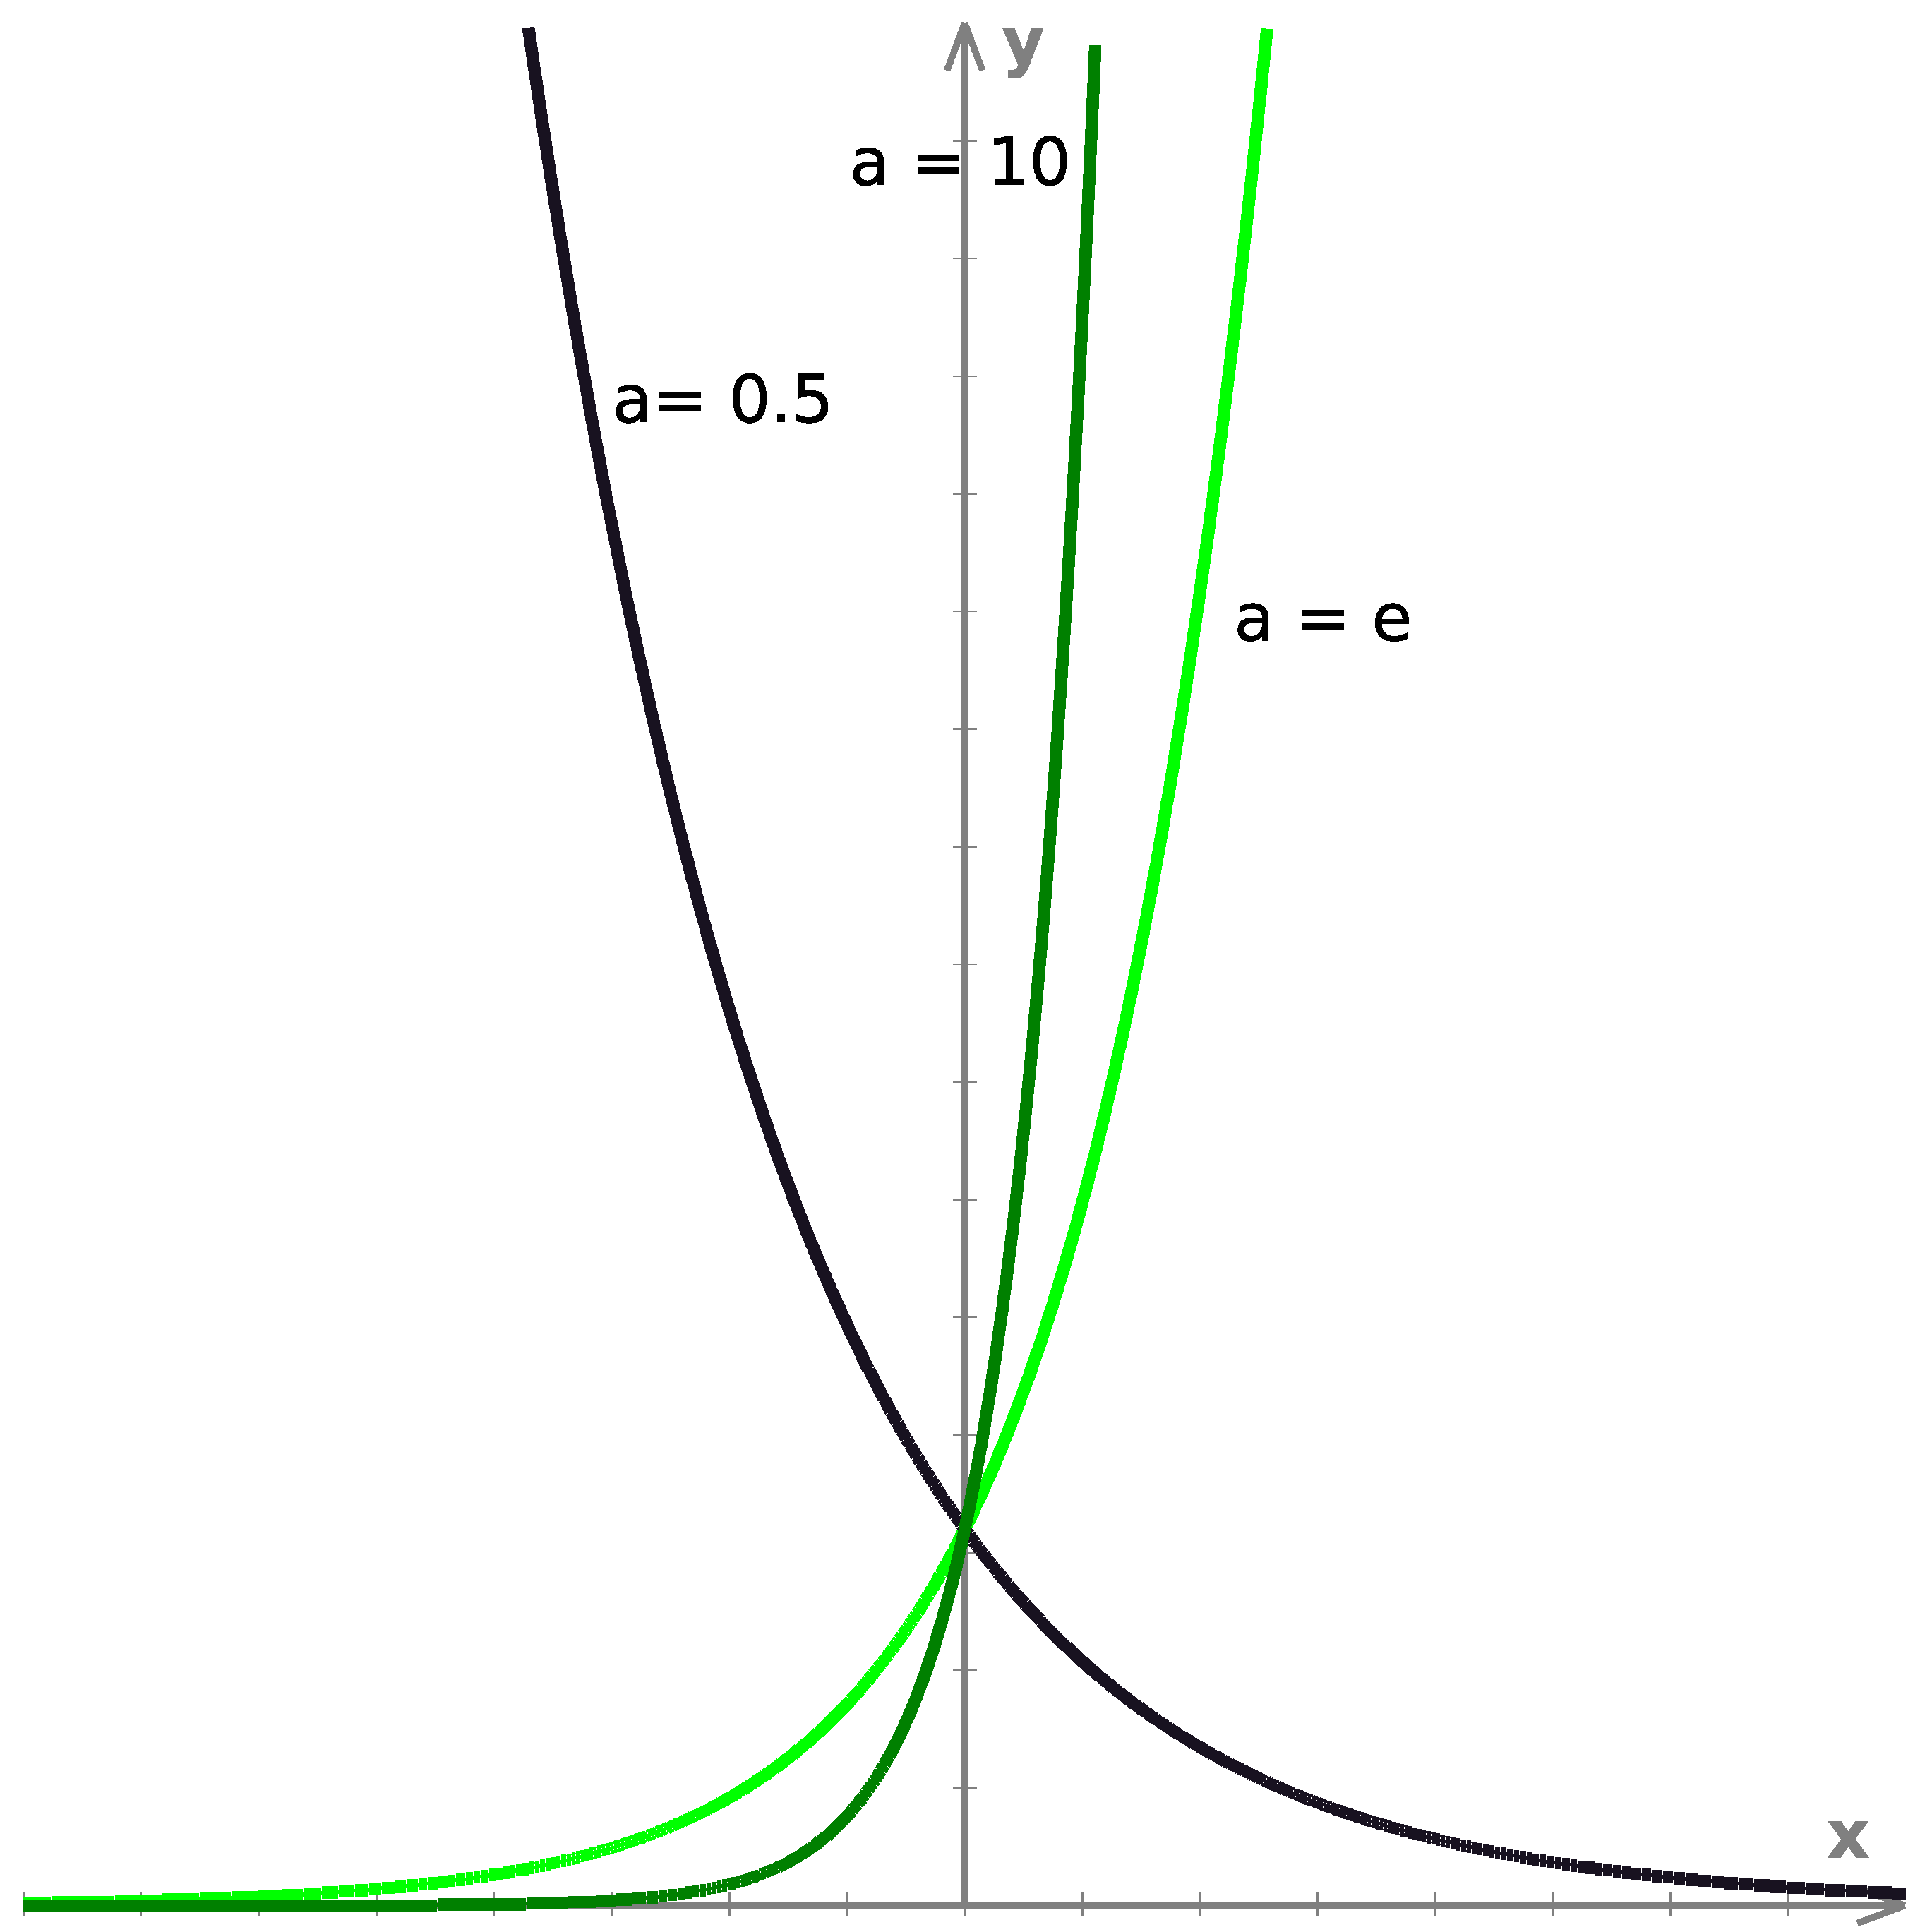
\includegraphics[height=4cm]{img/exp.pdf} 
\end{minipage}

\section*{Logarithmusfunktionen $y = \log_a x$ \\ mit $a \in
\mathbb{R_+}-\{1\}$}

\begin{minipage}{.5\textwidth}
\begin{itemize}
	\item \textbf{Definitionsbereich}: $ D = (0, + \infty) $
	\item \textbf{Wertebereich}: $ W = \mathbb{R} $
	\item \textbf{Nullstelle}: $ x_0 = 1 $
	\item \textbf{gemeinsamer Punkt}: $(1;0)$
	\item \textbf{Graph} für $a= e, 10, \tfrac{1}{2}$:
\end{itemize}
\end{minipage}
\begin{minipage}{.5\textwidth}
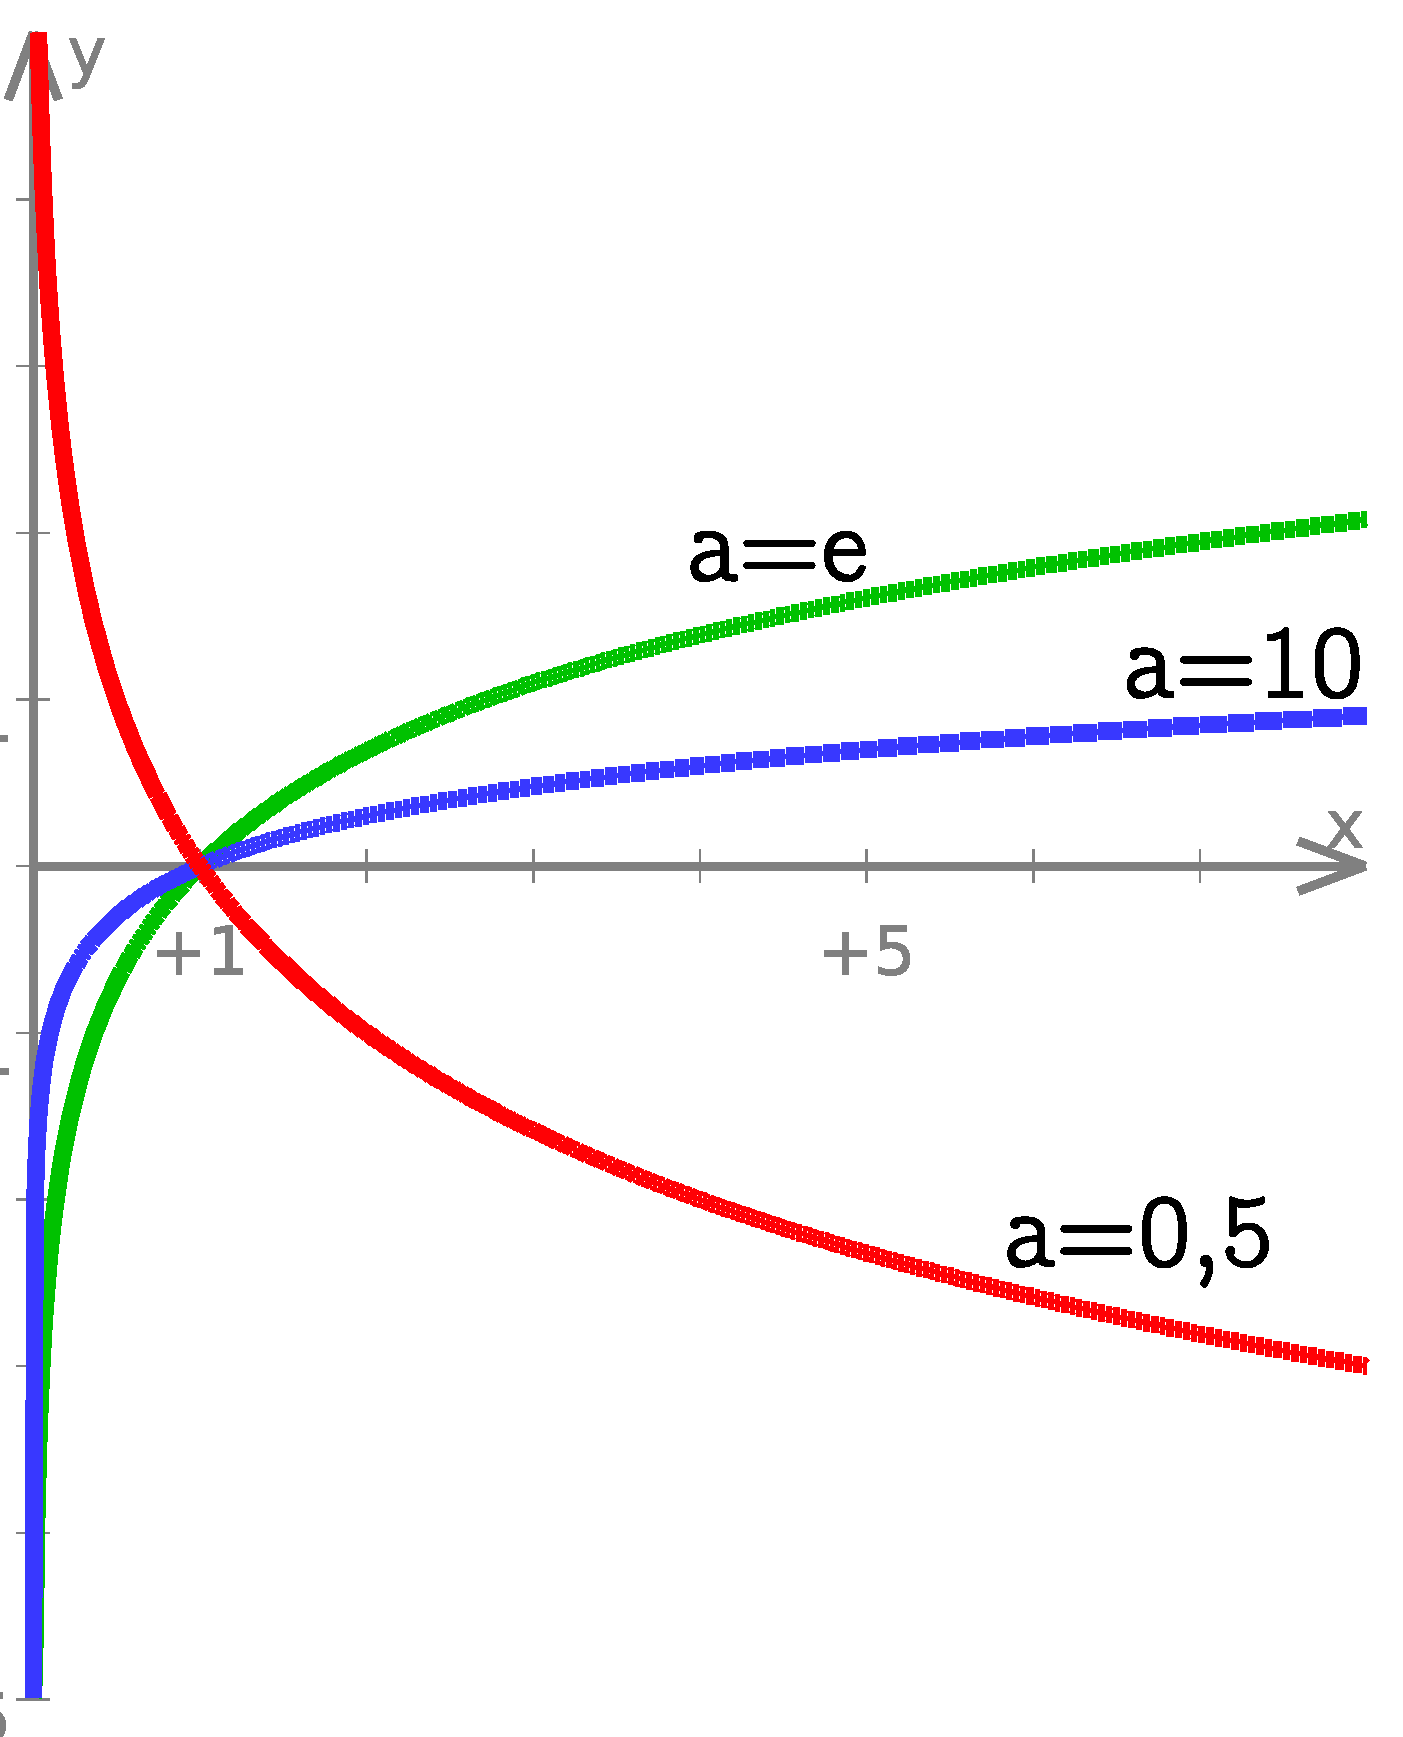
\includegraphics[height=4cm]{img/log.pdf}
\end{minipage}


%\section*{Literatur}
%Formeln und Tabellen für die Sekudarstufen I und II. 7. Aufl. - Berlin: Paetec, Ges. für %Bildung und Technik, 1999

